\documentclass[12pt,a4paper,oneside]{book}
\usepackage{helvet}
\renewcommand{\familydefault}{\sfdefault}
\usepackage[utf8]{inputenc}
\usepackage[T1]{fontenc}
\usepackage[spanish]{babel}
\usepackage{amsmath}
\usepackage{amsfonts}
\usepackage{amssymb}
\usepackage{graphicx}
\usepackage[left=2.5cm, right=4cm, top=5.00cm, bottom=2.50cm]{geometry}
\usepackage{eso-pic}
\usepackage{url}
\usepackage{microtype}
\setlength{\parindent}{0cm}
\usepackage{xhfill}
\usepackage{anysize}
\usepackage{apacite}
\usepackage{titletoc}
\usepackage{sectsty}
\chapternumberfont{\Large} 
\chaptertitlefont{\Large}
\sectionfont{\large}
\usepackage{setspace}
\usepackage[document]{ragged2e}
\usepackage{float}
\usepackage{booktabs, makecell, tabularx,array}
\newcolumntype{C}[1]{>{\centering\arraybackslash\hspace{0pt}}m{#1}}
{\renewcommand{\arraystretch}{0.8} % Espacios en blanco de filas en tablas
% Configuracion de los titulos y pie de tablas y figuras
\usepackage{caption} 
\captionsetup[table]{skip=10pt}
\captionsetup[table]{labelfont=bf,textfont=it}
\captionsetup[figure]{labelfont=bf,textfont=it}
\captionsetup{justification   = raggedright,
	singlelinecheck = false}

\newcommand\blfootnote[1]{%	
	\begingroup
	\renewcommand\thefootnote{}\footnote{#1}%
	\addtocounter{footnote}{-1}%
	\endgroup
}

\usepackage[pangram]{blindtext} % Texto random

\begin{document}

	
\begingroup
\begin{titlepage}
	\AddToShipoutPictureBG*{
		\AtPageUpperLeft{
			\raisebox{-\height}{
				\includegraphics[width=\paperwidth,height=\paperheight]{Port.pdf}
			}
		}
	}

	\begin{minipage}{\textwidth}
		\vspace{5cm}
		\noindent
		\begin{center}
			{\fontsize{14}{16}\ \textbf{DDDDDDDDDDDDDDDDDDDDDDDDDDDDDDDDDDDDDDD} \\[3\baselineskip]}
			
			{\fontsize{14}{16}\ \textbf{TESIS DE GRADO}\\[0.2\baselineskip]}
			
			{Que como requisito parcial para obtener el grado de:\\[0.4\baselineskip]}
			
			{\fontsize{14}{16}\ \textbf{MAESTRO EN INGENIERÍA AGRÍCOLA Y USO INTEGRAL DEL AGUA, ORIENTACIÓN EN MECANIZACIÓN AGRÍCOLA}\\[3\baselineskip]}
			
			{Presenta:\\[0.3\baselineskip]}
			
			{\textbf{CANEK MOTA DELFIN}\\[3\baselineskip]}
			
			{Bajo la supervisión de:\\[0.3\baselineskip]}
			
			{\textbf{dd}\\[8\baselineskip]}
			
			{Chapingo, Estado de México, agosto de 2022 }
			
		\end{center}
		
	\end{minipage}
\end{titlepage}
\endgroup


	\newpage
	\setcounter{page}{1}
	\renewcommand{\thepage}{\roman{page}}
	\pagestyle{plain}
	
\begin{large}
	\begin{center}
		\textbf{Titulo} 
	\end{center}
\end{large}


\vspace{1cm}
Tesis realizada por \textbf{Canek Mota Delfin} bajo la dirección del Comité Asesor indicado, aprobado por el mismo y aceptada como requisito parcial para obtener el grado de:

\vspace{1cm}
 \begin{center}
 	\textbf{MAESTRO EN INGENIERÍA AGRÍCOLA Y USO INTEGRAL DEL AGUA, ORIENTACIÓN EN MECANIZACIÓN AGRÍCOLA}
 \end{center}
\vspace{2cm}

DIRECTOR:\xrfill[1pt]{1pt}
\begin{center}
	Asesor

\end{center}
\vspace{2cm}

ASESOR:\xrfill[1pt]{1pt}
\begin{center}
	Asesor
	
\end{center}
\vspace{2cm}

ASESOR:\xrfill[1pt]{1pt}
\begin{center}
	Asesor
	
\end{center}
	\newpage
	\begin{large}
	\begin{center}
		\textbf{AGRADECIMIENTOS}
	\end{center}

\end{large}

	\newpage
	\begin{large}
	\begin{center}
		DATOS BIBLIOGRÁFICOS
	\end{center}

\end{large}

\vspace{2cm}
\begin{large}
	\begin{center}
		DATOS PERSONALES
	\end{center}
\end{large}


\begin{center}
	\begin{tabular}{p{5cm} p{7cm}}
		
		\textbf{Nombre} & Canek Mota Delfin \\
		\\
		\textbf{Fecha de nacimiento} & ddddd \\
		\\
		\textbf{Lugar de nacimiento} & ddddd \\
		\\
		\textbf{CURP} & dddd \\
		\\
		\textbf{Profesión} & Ingeniero Mecánico Agricola \\
		\\
		\textbf{Cédula profesional} & ddddd \\
		
	\end{tabular}

\end{center}
\vspace{.5cm}
\begin{large}
	\begin{center}
		DESARROLLO ACADÉMICO
	\end{center}

\end{large}


\begin{center}
	\begin{tabular}{p{5cm} p{7cm}}
		
		\textbf{Bachillerato:} & dddd  \\
		\\
		\textbf{Licenciatura:} & Universidad Autónoma Chapingo, Texcoco, Estado de México\\
	
		
	\end{tabular}
	
\end{center}
	
	\newpage
	\spacing{1.5}
	\renewcommand{\contentsname}{\centering CONTENIDO}
	\renewcommand{\tablename}{ Cuadro}
	\renewcommand{\listtablename}{ \centering LISTA DE CUADROS}
	\renewcommand{\listfigurename}{ \centering LISTA DE FIGURAS}
	
	\tableofcontents
	\listoftables
	\listoffigures
	
	\newpage
	
\section*{\centering RESUMEN GENERAL}
\addcontentsline{toc}{section}{RESUMEN GENERAL}
\justify
\microtypesetup{activate=true}

\begin{center}
	GGGGGGGGGGGGGGGGGGGGGGGGGGGGG
\end{center}
\hfill \break


\blindtext
\blindtext

\textbf{Palabras claves}:

\blfootnote{Tesis de Maestría en Ingeniería Agrícola y Uso Integral del Agua (IAUIA) }
\blfootnote{Universidad Autónoma Chapingo}
\blfootnote{Autor: }
\blfootnote{Director de Tesis: }
	\newpage
	
\section*{\centering GENERAL ABSTRACT}
\addcontentsline{toc}{section}{GENERAL ABSTRACT}

\blindtext
\blindtext

\textbf{Keywords}: 


\blfootnote{Thesis}
\blfootnote{Author:}
\blfootnote{Advisor:}

	\newgeometry{left=4.00cm, right=2.50cm, top=2.50cm, bottom=2.50cm}
	\renewcommand{\thepage}{\arabic{page}}
	\newpage
	
	\chapter{INTRODUCCIÓN GENERAL}
\section{INTRODUCCIÓN}

\Blindtext


\section{OBJETIVO GENERAL}
\blindtext
\section{OBJETIVOS PARTICULARES}

\begin{itemize}
	\item Planificar 
\end{itemize}
	\chapter{REVISIÓN DE LITERATURA}

\blindmathpaper

\begin{figure}[H] % tiny 
	\centering
	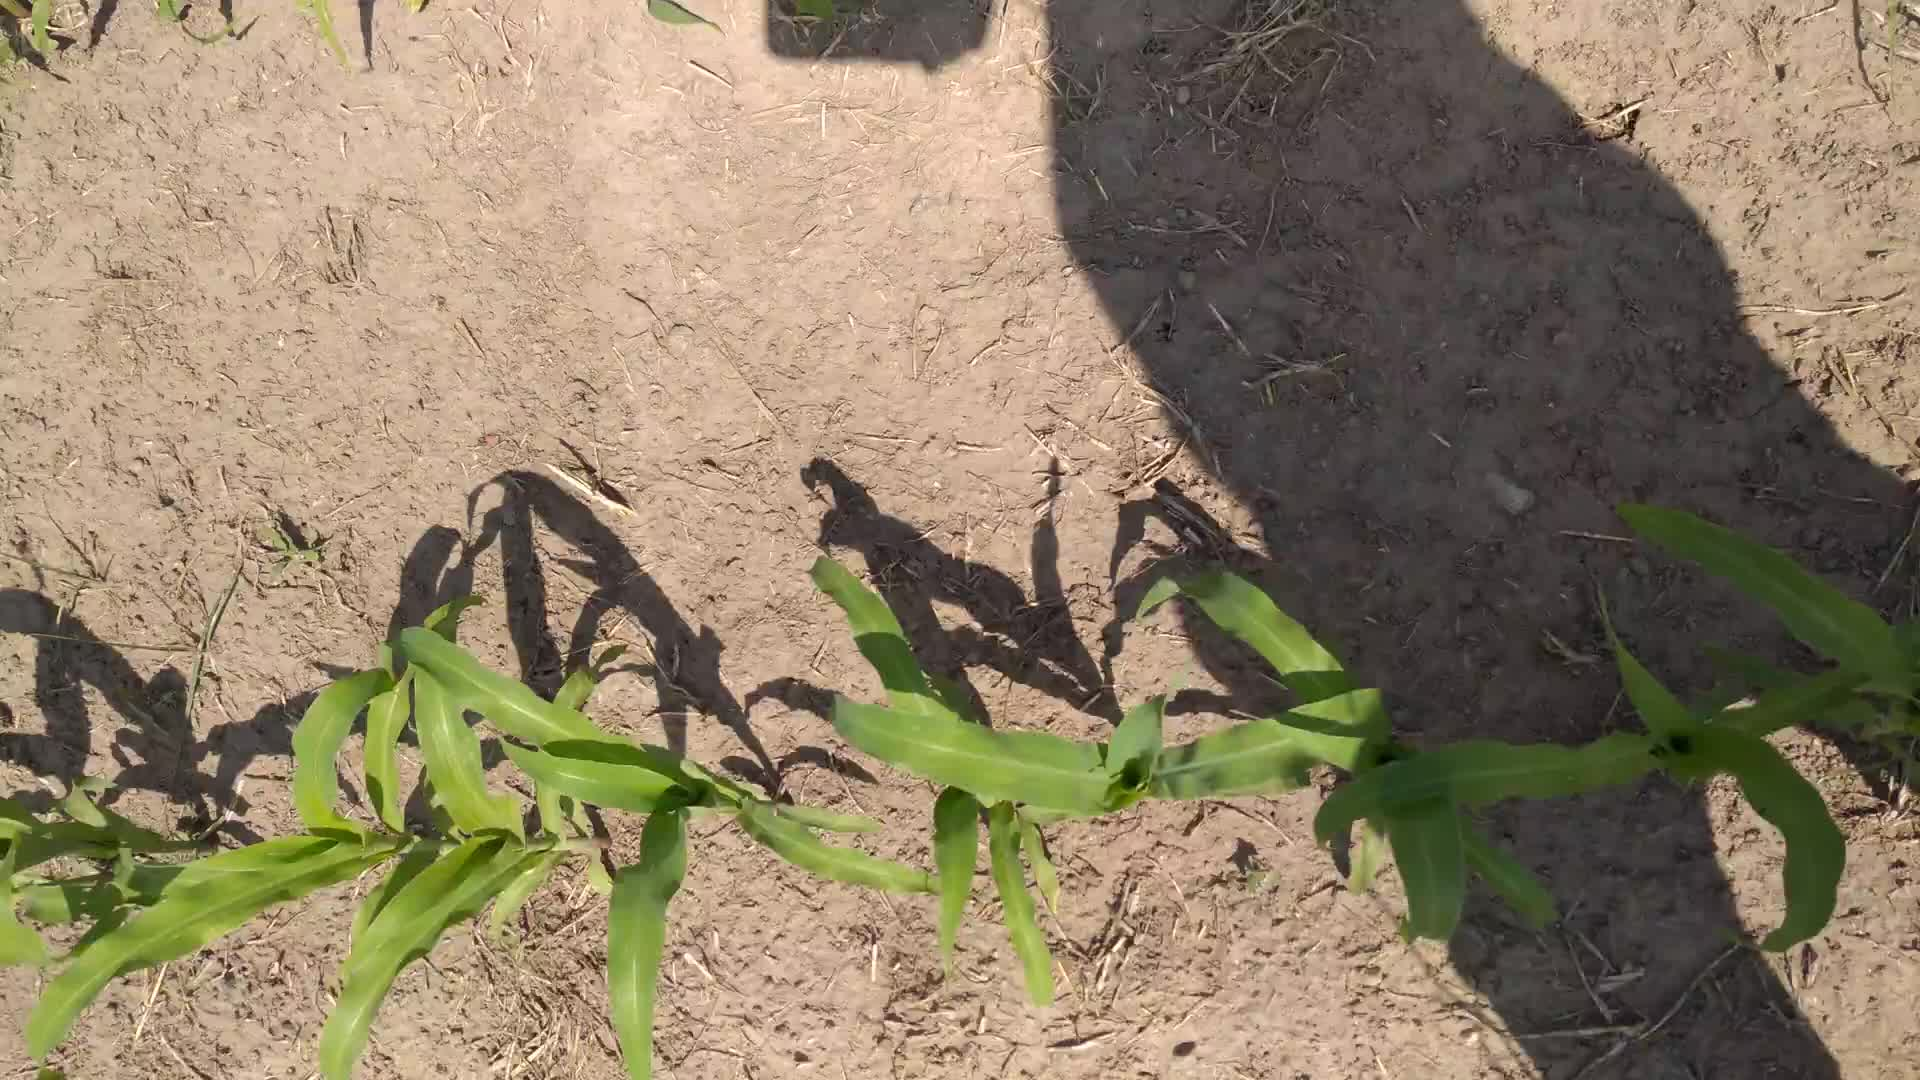
\includegraphics[width=1\textwidth]{Imagenes/0001}
	\caption[Titulo de lista]{Titulo completo}
	\label{fig:yolov4-t}
\end{figure}


\begin{table}[H] % versiones de YOLOv5
	\caption[Versiones de YOLOv5]{Versiones de YOLOv5} \label{tab:Verv5}
	\centering
	\begin{tabular}{lcc}
		\toprule
		\textbf{Versión} & \textbf{Profundidad del modelo} & \textbf{Ancho de capas}\\
		\midrule
		YOLOv5n & 0.33 & 0.25 \\
		YOLOv5s & 0.33 &  0.50 \\
		YOLOv5m & 0.67 & 0.75 \\
		YOLOv5l & 1.00 & 1.00 \\
		YOLOv5x & 1.25 & 1.25 \\
		\bottomrule
	\end{tabular}
\end{table}
	\chapter{ARTÍCULO CIENTÍFICO}

\blindmathpaper
	\newpage
	\bibliographystyle{apacite}
	\bibliography{Bibliografia.bib}
	
	
\end{document}